\documentclass{beamer}
\usepackage{hyperref}

% other packages
\usepackage{latexsym,amsmath,xcolor,multicol,booktabs,calligra}
\usepackage{graphicx,pstricks,listings,stackengine}

% packages and settings for bibtex
\usepackage[backend=bibtex,sorting=none]{biblatex}
\addbibresource{ref.bib}
\setbeamerfont{footnote}{size=\tiny}   % footnote for bibtex
\setbeamertemplate{bibliography item}[text]   % reference list for bibtex
\defbibheading{reference}{\section*{Reference}}   % heading for bibtex

\author[Yves R. Sagaert]{Yves R. Sagaert (title slide) \\{\small yves.sagaert@vives.be}}
\title{VIVES Business Management Theme}
\subtitle{Subtitle}
\institute{VIVES University of Applied Sciences }
\date{\today} 
\usepackage{vivesbm}

% defs
\def\cmd#1{\texttt{\color{red}\footnotesize $\backslash$#1}}
\def\env#1{\texttt{\color{blue}\footnotesize #1}}
\definecolor{deepblue}{rgb}{0,0,0.5}
\definecolor{deepred}{rgb}{0.6,0,0}
\definecolor{deepgreen}{rgb}{0,0.5,0}
\definecolor{halfgray}{gray}{0.55}

\lstset{
    basicstyle=\ttfamily\small,
    keywordstyle=\bfseries\color{deepblue},
    emphstyle=\ttfamily\color{deepred},    % Custom highlighting style
    stringstyle=\color{deepgreen},
    numbers=left,
    numberstyle=\small\color{halfgray},
    rulesepcolor=\color{red!20!green!20!blue!20},
    frame=shadowbox,
}


\begin{document}
% Title slide
\begin{frame}
    \titlepage
    \begin{figure}[htpb]
        \begin{center}
            %\includegraphics[width=0.15\linewidth]{fig/KUL.eps}\quad\quad\quad\quad
            
\includegraphics[width=0.35\linewidth]{fig/vives_logo2022.png}
        \end{center}
    \end{figure}
\end{frame}   
\begin{frame}
    \tableofcontents[sectionstyle=show,subsectionstyle=show/shaded/hide,subsubsectionstyle=show/shaded/hide]
\end{frame}


\section{Section 1}

\begin{frame}{Latex template}
    \begin{itemize}[<+-| alert@+>] 
        \item one
        \item two
    \end{itemize}
\end{frame}


\section{Section 2}

\subsection{Examples}

\begin{frame}{Frametitle}
    \begin{itemize}
        \item one
        \item two
        \begin{enumerate}
            \item one
            \item two
        \end{enumerate}
    \end{itemize}
\end{frame}


\section{Section 3}

\subsection{More?}



\begin{frame}{Math}
    \begin{exampleblock}{Good equation here} 
        \begin{equation*}
            J(\theta) = \mathbb{E}_{\pi_\theta}[G_t] = \sum_{s\in\mathcal{S}} d^\pi (s)V^\pi(s)=\sum_{s\in\mathcal{S}} d^\pi(s)\sum_{a\in\mathcal{A}}\pi_\theta(a|s)Q^\pi(s,a)
        \end{equation*}
    \end{exampleblock}
    \begin{exampleblock}{More stuff\footnote{unreadable}}
        
        \begin{align}
            Q_\mathrm{target}&=r+\gamma Q^\pi(s^\prime, \pi_\theta(s^\prime)+\epsilon)\\
            \epsilon&\sim\mathrm{clip}(\mathcal{N}(0, \sigma), -c, c)\nonumber
        \end{align}
    \end{exampleblock}
\end{frame}

\begin{frame}
    \begin{exampleblock}{Totally logical example}
        % Taken from Mathmode.tex
        \begin{multline}
            A=\lim_{n\rightarrow\infty}\Delta x\left(a^{2}+\left(a^{2}+2a\Delta x+\left(\Delta x\right)^{2}\right)\right.\label{eq:reset}\\
            +\left(a^{2}+2\cdot2a\Delta x+2^{2}\left(\Delta x\right)^{2}\right)\\
            +\left(a^{2}+2\cdot3a\Delta x+3^{2}\left(\Delta x\right)^{2}\right)\\
            +\ldots\\
            \left.+\left(a^{2}+2\cdot(n-1)a\Delta x+(n-1)^{2}\left(\Delta x\right)^{2}\right)\right)\\
            =\frac{1}{3}\left(b^{3}-a^{3}\right)
        \end{multline}
    \end{exampleblock}
\end{frame}

\begin{frame}{Graphical example}
    % From thuthesis user guide.
    \begin{minipage}[c]{0.3\linewidth}
        \psset{unit=0.8cm}
        \begin{pspicture}(-1.75,-3)(3.25,4)
            \psline[linewidth=0.25pt](0,0)(0,4)
            \rput[tl]{0}(0.2,2){$\vec e_z$}
            \rput[tr]{0}(-0.9,1.4){$\vec e$}
            \rput[tl]{0}(2.8,-1.1){$\vec C_{ptm{ext}}$}
            \rput[br]{0}(-0.3,2.1){$\theta$}
            \rput{25}(0,0){%
            \psframe[fillstyle=solid,fillcolor=lightgray,linewidth=.8pt](-0.1,-3.2)(0.1,0)}
            \rput{25}(0,0){%
            \psellipse[fillstyle=solid,fillcolor=yellow,linewidth=3pt](0,0)(1.5,0.5)}
            \rput{25}(0,0){%
            \psframe[fillstyle=solid,fillcolor=lightgray,linewidth=.8pt](-0.1,0)(0.1,3.2)}
            \rput{25}(0,0){\psline[linecolor=red,linewidth=1.5pt]{->}(0,0)(0.,2)}
%           \psRotation{0}(0,3.5){$\dot\phi$}
%           \psRotation{25}(-1.2,2.6){$\dot\psi$}
            \psline[linecolor=red,linewidth=1.25pt]{->}(0,0)(0,2)
            \psline[linecolor=red,linewidth=1.25pt]{->}(0,0)(3,-1)
            \psline[linecolor=red,linewidth=1.25pt]{->}(0,0)(2.85,-0.95)
            \psarc{->}{2.1}{90}{112.5}
            \rput[bl](.1,.01){C}
        \end{pspicture}
    \end{minipage}\hspace{1cm}
    \begin{minipage}{0.5\linewidth}
        \medskip
        %\hspace{2cm}
        \begin{figure}[h]
            \centering
            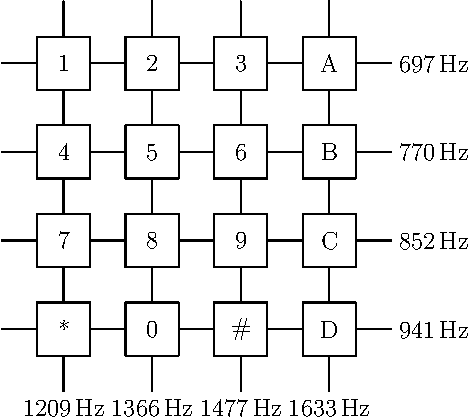
\includegraphics[height=.4\textheight]{fig/dtmf.pdf}
        \end{figure}
    \end{minipage}
\end{frame}

\begin{frame}{Slide with citations in slide}
    ResNet\footfullcite{he2016deep}, Transformer\footfullcite{vaswani2017attention},
    \ref{fig:transformer-arc}
    \begin{figure}[htbp]
        \centering
        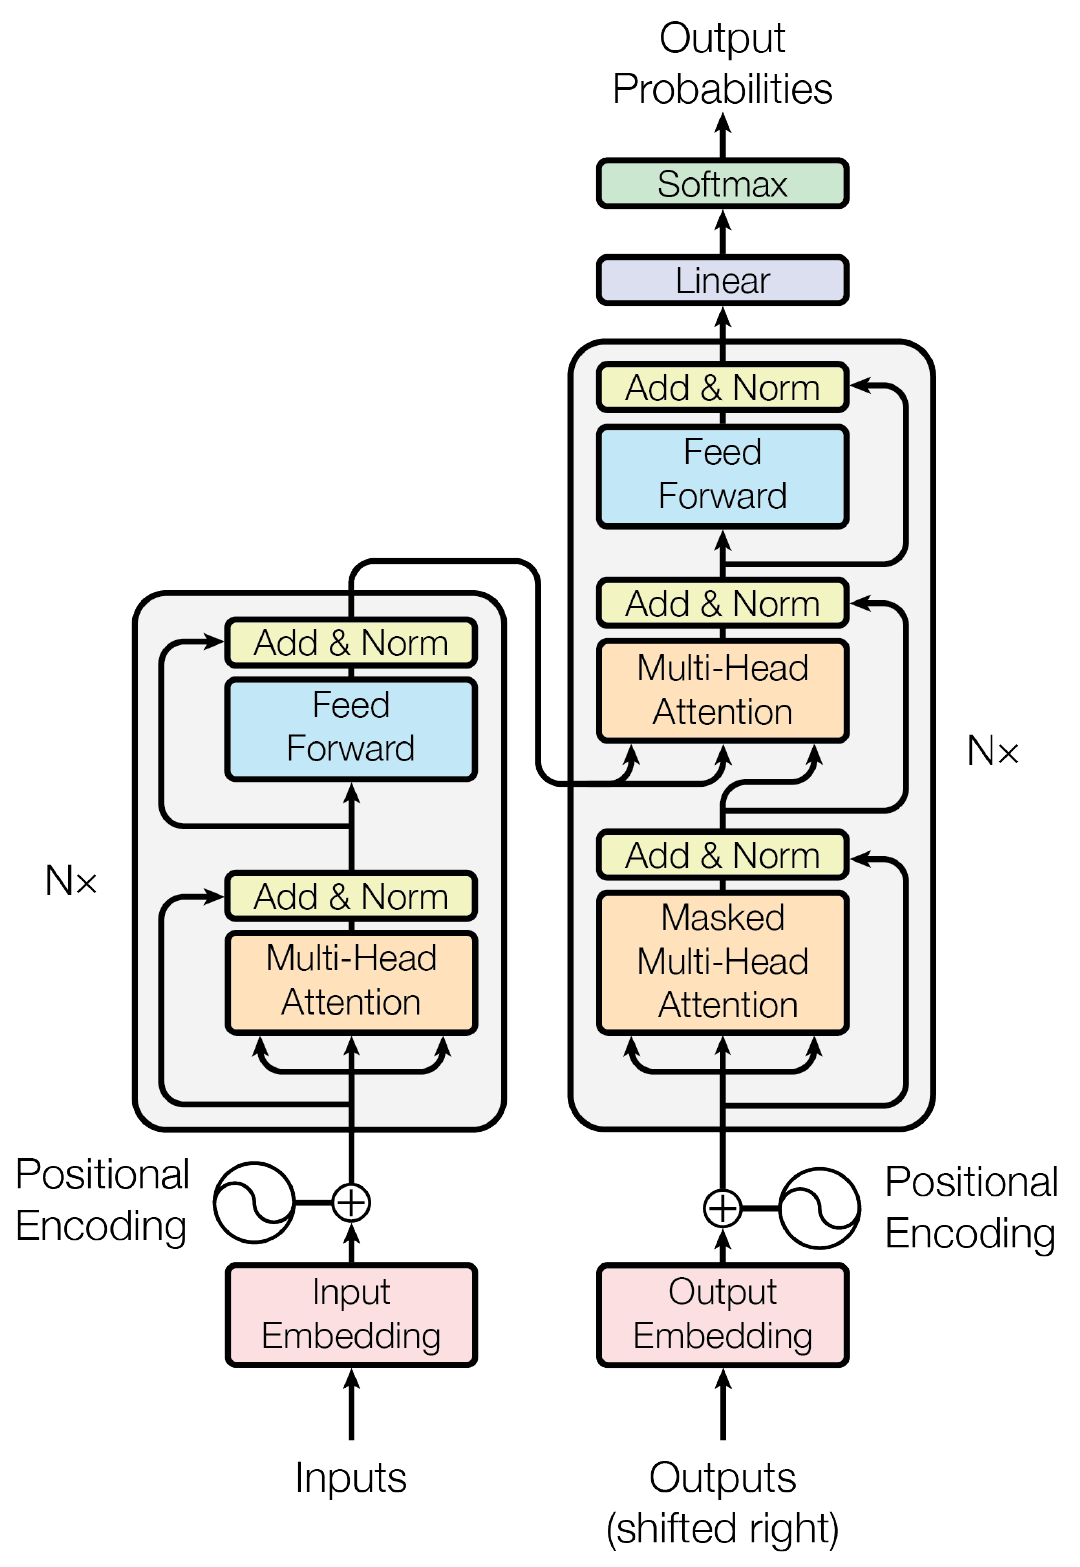
\includegraphics[width=0.25\textwidth]{fig/transformer_arch.png}
        \caption{Transformer figure}
        \label{fig:transformer-arc}
    \end{figure}
\end{frame}

\begin{frame}[fragile]{\LaTeX{} Commands}
    \begin{exampleblock}{Most used}
        \centering
        \footnotesize
        \begin{tabular}{llll}
            \cmd{chapter} & \cmd{section} & \cmd{subsection} & \cmd{paragraph} \\
            title & section & subtitle & par \\\hline
            \cmd{centering} & \cmd{emph} & \cmd{verb} & \cmd{url} \\
            outline & bold & italic & link \\\hline
            \cmd{footnote} & \cmd{item} & \cmd{caption} & \cmd{includegraphics} \\
            footnote & bullets & cap & figure \\\hline
            \cmd{label} & \cmd{cite} & \cmd{ref} \\
            set to ref & citation & ref in document\\\hline
        \end{tabular}
    \end{exampleblock}
    \begin{exampleblock}{Also interesting}
        \centering
        \footnotesize
        \begin{tabular}{lll}
            \env{table} & \env{figure} & \env{equation}\\
            table & fig & eq \\\hline
            \env{itemize} & \env{enumerate} & \env{description}\\
            bullets & numbers & descr. \\\hline
        \end{tabular}
    \end{exampleblock}
\end{frame}

\begin{frame}[fragile]{\LaTeX{} Code block explained}
    \begin{minipage}{0.5\linewidth}
\begin{lstlisting}[language=TeX]
\begin{itemize}
  \item A \item B
  \item C
  \begin{itemize}
    \item C-1
  \end{itemize}
\end{itemize}
\end{lstlisting}
    \end{minipage}\hspace{1cm}
    \begin{minipage}{0.3\linewidth}
        \begin{itemize}
            \item A
            \item B
            \item C
            \begin{itemize}
                \item C-1
            \end{itemize}
        \end{itemize}
    \end{minipage}
    \medskip
    \pause
    \begin{minipage}{0.5\linewidth}
\begin{lstlisting}[language=TeX]
\begin{enumerate}
  \item 1 \item 2
  \item 3
  \begin{itemize}
    \item[n+e] 4
  \end{itemize}
\end{enumerate}
\end{lstlisting}
    \end{minipage}\hspace{1cm}
    \begin{minipage}{0.3\linewidth}
        \begin{enumerate}
            \item 1
            \item 2
            \item 3
            \begin{itemize}
                \item[n+e] 4
            \end{itemize}
        \end{enumerate}
    \end{minipage}
\end{frame}


\section{End section}
\begin{frame}
    \begin{itemize}
        \item Thanks for your attention
        \item Use this template
    \end{itemize}
\end{frame}

% \section{References}

% \begin{frame}[allowframebreaks]
%     %\bibliography{ref}
%     \bibliographystyle{alpha}
%     % a,b :
%     % \tiny\bibliographystyle{alpha}
% \end{frame}

\begin{frame}{References}
	\printbibliography[heading=reference]
\end{frame}

\begin{frame}
    \begin{center}
        {\Huge\calligra That's all folks!\\Thanks!}
    \end{center}
\end{frame}

\end{document}